\chapter{Error computation\label{chap:error}}
\vspace*{-1cm}
\lettrine[lines=2, loversize=-0.1, lraise=0.1]{D}{iva} 

\minitoc


\section{Introduction}

% \section{Error field with advection}

% provided by diva, but interpretation different as the normal case
% need to add more details on this
The analysis performed with the optimised parameters should have the lowest global error, as measured by \eqref{eq:gcvbis}. Nevertheless, the spatial distribution of the error is also of interest. The latter is very easy to calculate with OI: according to \eqref{eq:erroroi} we need to apply the analysis (operator $\matr{H}$) on a vector containing the covariances of the data locations with the location where the error has to be calculated. Hence, in principle, a new analysis has to be performed for each point in which the error is requested. On the contrary, the error calculation in \diva is not trivial since the covariance functions are never explicitly specified. The object of this section is to define methods to generate error fields associated to the analysis. 

\subsection{The poor man's estimate}

To circumvent the main problems (unknown covariance function and repeated analysis), \citet{BRASSEUR94} estimated the error by analysing a vector of "covariances" with constant $\sigma^2$. As all "covariances" are identical, the error can be assessed in all locations with the same analysis. The advantage is the fast calculation, but the drawback is a systematic underestimation of the actual errors, since the error reduction by the overestimated covariances \eqref{eq:erroroi} is also overestimated. The poor man's error field is a very efficient way to assess data-coverage and determine the regions where the analysis cannot be trusted.

\subsection{The hybrid approach}

In this approach, the covariance vector to be analysed is calculated using the covariance function of an infinite domain \citep{BRANKART98,RIXEN00}. In an infinite domain, the error calculation is then "exact", while for more complicated domains, it is nearly exact far away from boundaries, provided no anisotropic constraint is activated. 

The problem of the approximate hybrid error calculation relies on the fact that instead of the actual covariance, only the kernel computed under the assumption of an infinite domain (without dynamic constrain) is analysed with \diva to produce the error field. Hence, for anisotropic cases (as found with advection constraints, variable length scale or near boundaries), the hybrid error field can be incoherent. This is what motivated the evaluation of the real covariance function in \diva.

\subsection{The real covariance method}

If we look back at the OI interpretation, we can place a data of value $1$ at location $\vect{r}$ and compute the analysis $\varphi_1(\vect{r}^\prime)$ at a location $\vect{r}^\prime$:
\begin{equation}
\varphi_1(\vect{r}^\prime) = {\snr \hat{B} (\vect{r},\vect{r}^\prime)\over  \snr \hat{B}(\vect{r},\vect{r}) + \hat{R}(\vect{r}) },
\end{equation}
where $\hat{B}(\vect{r},\vect{r}^\prime)$ is the non-dimensional covariance function between points $\vect{r}$ and $\vect{r}^\prime$, whereas $\hat{R}$ is the normalized observational error variance. Normalization was done respectively by the background variance $\sigma^2$ and noise $\noise^2$, yielding the signal-to-noise ratio $\snr$ previously defined. 
At the data location itself, we get the analysis
\begin{equation}
\varphi_1(\vect{r}) = {\snr \hat{B} (\vect{r},\vect{r}) \over \snr \hat{B}(\vect{r},\vect{r}) + \hat{R}(\vect{r}) }.
\end{equation}

In terms of interpretation of the covariance function as the kernel of the norm (the second term of \eqref{eq:variab}), it is the background covariance that is modified by the anisotropy and not the noise level. Hence, if we put the unit data value with a unit signal-to-noise ratio in $\vect{r}$, we directly have

\begin{equation}
\varphi_1(\vect{r}^\prime) = { \hat{B} (\vect{r},\vect{r}^\prime)\over   \hat{B}(\vect{r},\vect{r}) + 1 } \qquad \textrm{and} \qquad 
\varphi_1(\vect{r}) = { \hat{B} (\vect{r},\vect{r}) \over  \hat{B}(\vect{r},\vect{r}) + 1 }.
\end{equation}
The left-hand sides are provided by the \diva application to the unit data point in location $\vect{r}$ with unit signal-to-noise ratio and analysed in any desired location $\vect{r}^\prime$ and $\vect{r}$. From these two values, it is therefore easy to calculate the covariance function $\hat{B}$ inherently used in \diva.

For the error calculation at a point $\vect{r}$, we have the following procedure: 

\begin{enumerate}

\item Put a unit value at $\vect{r}$ and perform an analysis with $\snr=1$.

\item Save the result at the locations of the original data and of the error-calculation, where the analysis value is
\begin{equation}
\varphi_0 ~=~{ \hat{B} (\vect{r},\vect{r}) \over \hat{B}(\vect{r},\vect{r}) + 1 },
\end{equation}

\item Calculate the background variance $\hat{B}(\vect{r},\vect{r})$ at the error-field location:
\begin{equation}
\hat{B} (\vect{r},\vect{r}) = { \varphi_0 \over 1 - \varphi_0}.
\label{eq:brr}
\end{equation}

\item Calculate the covariance $\hat{B} (\vect{r},\vect{r}_i)$ between the error location and data locations. Since at the data points $i$ located at $\vect{r}_i$, \diva application provides
\begin{equation}
\varphi_i ~=~ { \hat{B} (\vect{r},\vect{r}_i) \over \hat{B}(\vect{r},\vect{r}) + 1 },
\end{equation}
the covariance $\hat{B} (\vect{r},\vect{r}_i)$ is obtained as
\begin{equation}
\hat{B} (\vect{r},\vect{r}_i)~=~{\varphi_i \over ( 1-\varphi_0 )}.
\label{eq:btildco}
\end{equation}

\end{enumerate}

Up to the multiplication constant $1/(1-\varphi_0)$, the non-dimensional covariance of a point in position $\vect{r}$ with a list of other points can therefore be obtained by putting a unit data value in $\vect{r}$ and taking the value of the analysis at the coordinates of the list of points. 


To illustrate the procedure, we take a simple case with one point in the center of the domain, and another point near the boundary.
Near the boundary, data points influence more easily the analysis because rigidity is reduced (Fig.~\ref{fig:fig4_kernel_bceffect}). This translates into a larger background variance. Error fields will therefore be larger near boundaries when there are no nearby data.
 
\begin{figure}[htpb]
\centering
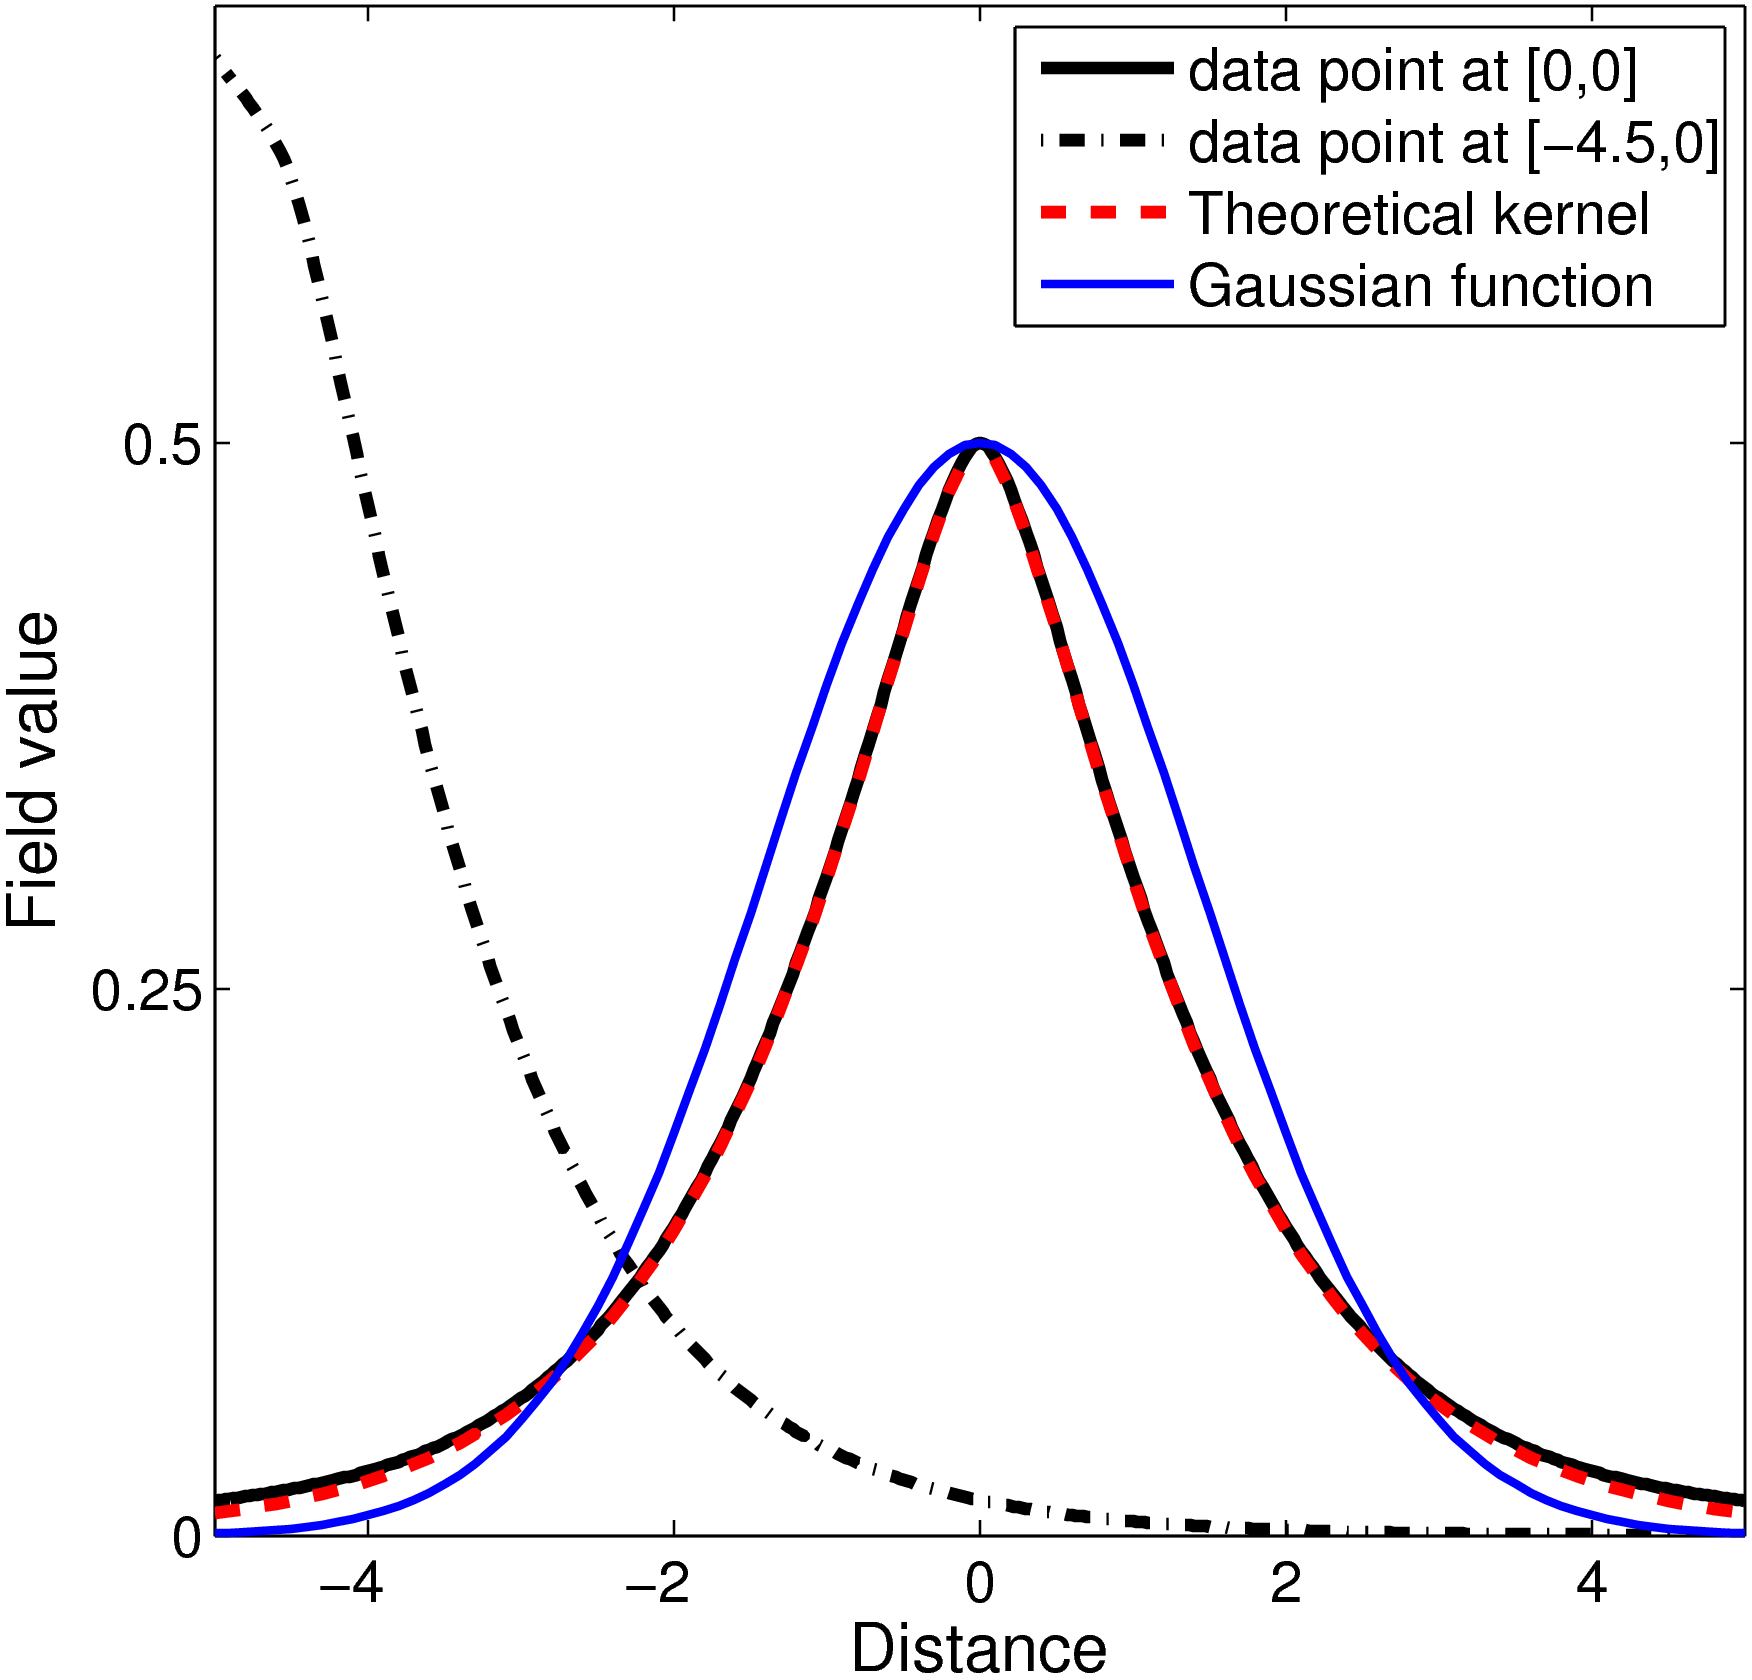
\includegraphics[width=.7\textwidth,bb=66 206 510 630]{fig4_kernel_bceffect}
\caption{Analysis in a square domain $[-5,5]\times[-5,5]$ with a point at the centre and another at $(-4.5,0)$. The signal-to-noise ratio $\snr=1$ for both cases. Note the larger analysis value near the boundary, indicating a larger background variance.
\label{fig:fig4_kernel_bceffect}}
\end{figure} 
 
 
From there, applying the correction $1/(1-\varphi_0)$, we can use the covariances as input vector for a second \diva execution, so as to perform an analysis of the covariance and getting access to the error of the analysis at the desired location. Indeed, using the equivalence of \diva and OI, if the analysis step applied to a data vector $\vect{d}$ is formally written 
\begin{equation}
\varphi_a = \matr{H} \vect{d},
\end{equation}
then the error is 
\begin{equation}
\epsilon_a^2 (\vect{r}) = \sigma^2 \hat{B}(\vect{r},\vect{r}) - \sigma^2 \matr{H} \hat{\vect{b}},
\end{equation}
where $\hat{B}(\vect{r},\vect{r})$ is the local relative background variance (calculated by \eqref{eq:brr}) and $\hat{\vect{b}}$ is a vector filled according to \eqref{eq:btildco}.

\subsubsection{Error on integral of a field}

The calculation of covariances can also be exploited to derive the error committed in the evaluation of the integral of the analysed field (for instance heat or salt content) over the whole domain or a sub-domain. 

% Add content of divaintegral.tex